
\section{Force, energy, work}
The argument is\footnote{Taylor ch. 4}:

\begin{enumerate}
\item Suppose a particle is moving under the influence of a force, according to Newton's Second Law.
\item Consider the integral of the force over some section of the particle's trajectory:
  $\int_{\vec{r_0 \to \vec{r_1}}} F(\vec{r}) \dif \vec{r}$.
\item The integral is equal to the difference in value of a certain quantity that depends on speed,
  evaluated at the start and end point.
\item This quantity is $\frac{1}{2}mv^2$. It depends only on the particle's mass, and speed at a
  moment in time. As long as the particle's motion obeys Newton's Second Law
  $m\ddot{\vec{r}} = F(\vec{r})$, then the relationship between this quantity and the integral of
  force over space is just a fact of calculus.
\item The quantity $\frac{1}{2}mv^2$ is given the name \blue{kinetic energy} and the integral of
  force over a path in space is given the name \blue{work}.
\item Thus the \blue{Work - KE Theorem}: when a particle is moved along a path according to Newton's
  Second Law, then the work done by the force is equal to the difference in kinetic energy.
\item This can be used, for example, to calculate the new velocity, given knowledge of the work done
  and the initial velocity.
\item So the work done when moving from $\vec{r_0}$ to $\vec{r}$ is equal to the difference in
  kinetic energy at those locations\footnote{This implies that every position is associated with a
    unique speed?}:
  \begin{align*}
    W(\vec{r_0} \to \vec{r})
    &= \int_{\vec{r_0}}^{\vec{r}} F(\vec{r}) \dif \vec{r} \\
    &= \frac{1}{2}mv^2 - \frac{1}{2}mv_0^2.
  \end{align*}
\item Therefore the following quantity is constant at all points along the path:
  \begin{align*}
    E
    &= \frac{1}{2}mv^2 - \int_{\vec{r_0}}^{\vec{r}} F(\vec{r}) \dif \vec{r} \\
    &= \frac{1}{2}mv_0^2.
  \end{align*}
\end{enumerate}


Suppose we start at position $x_0$ with speed $v_0$. Some time later we find ourselves at position
$x_1$ with speed $v_1$. Then the change in our KE is equal to the work done by the force along the
path we followed, $T(v_1) - T(v_0) = W(x_0 \to x_1)$. So, for this path, we have that the quantity
\begin{align*}
  T(v_1) - W(x_0 \to x_1)
\end{align*}
is constant and equal to $T(v_0)$.


Now suppose that in this system the work done along any path depends only on the endpoints of the
path, and not otherwise on the actual path followed. Then the quantity
\begin{align*}
  T(v) - W(x_0 \to x)
\end{align*}
is constant, where $v$ is the speed at $x$.

{\bf Intuition:} the quantity that is conserved is
\begin{align*}
  \text{(new KE at some position)} - \text{(change in KE that must have occurred to get there)}
\end{align*}



\subsection{Non-mathematical explanation of potential energy and kinetic energy}

Suppose we're in a 1-dimensional universe (i.e our universe is just one straight line). There's a
force that's pushing to the left or to the right, with some strength, at every point along the
line. The force doesn't vary over time; it depends only on where we are along the line. And there's
no friction; the only thing accelerating us (in one direction or the other) is the force.

% We're going to be moved around under the influence of the force; apart from the force, there's
% nothing else that will make us move, and we can't prevent the force moving us.

Let $x$ be our location on the line, and let $F(x)$ be the value of the force at that location
(negative means it's pushing to the left).

We're going to keep track of how much force we are subject to while it moves us around. So, we keep
a running total of all the $F$ values we are subject to at all the locations along the line that we
are taken to. If the force is pushing to the right with some strength $F$ then our running total
goes up by $F$; if it's pushing to the left, then it goes down by $F$. Then, at the new location we
were taken to, we do the same thing according to the strength of the force there. Except, of course,
space is continuous and this doesn't really happen in discrete steps: instead we compute the
integral of the $F$ function over some region of the line.

Let $V(x)$ be the value of this integral, i.e. the net amount of force we encounter while being
moved from our starting position to some position $x$. Recall that, basically, force is something
that causes acceleration. In other words, it increases or decreases our velocity. So $E$ is in some
sense measuring our net gain in velocity as we move around the line.

Now, suppose we're at some point $x_0$ on the line. The force is pushing us to the right. Looking to
the right, the value of the force function over that region dictates that a certain change in our
velocity will occur while we traverse it. So there's some function $V(x)$ that says, if the force
moves us to $x$, how much change in our velocity this will result in.

Say we start of at $a$ with some amount $T$ of velocity.

So that's like a promised amount of
change.


The function that maps $x$ to the
change in velocity that will occur between here and $x$ is called the potential energy function
$V(x)$.

\subsection{Solving a gravity problem using dimensional analysis, Newton's Second Law, and Conservation of Energy}

\begin{mdframed}
  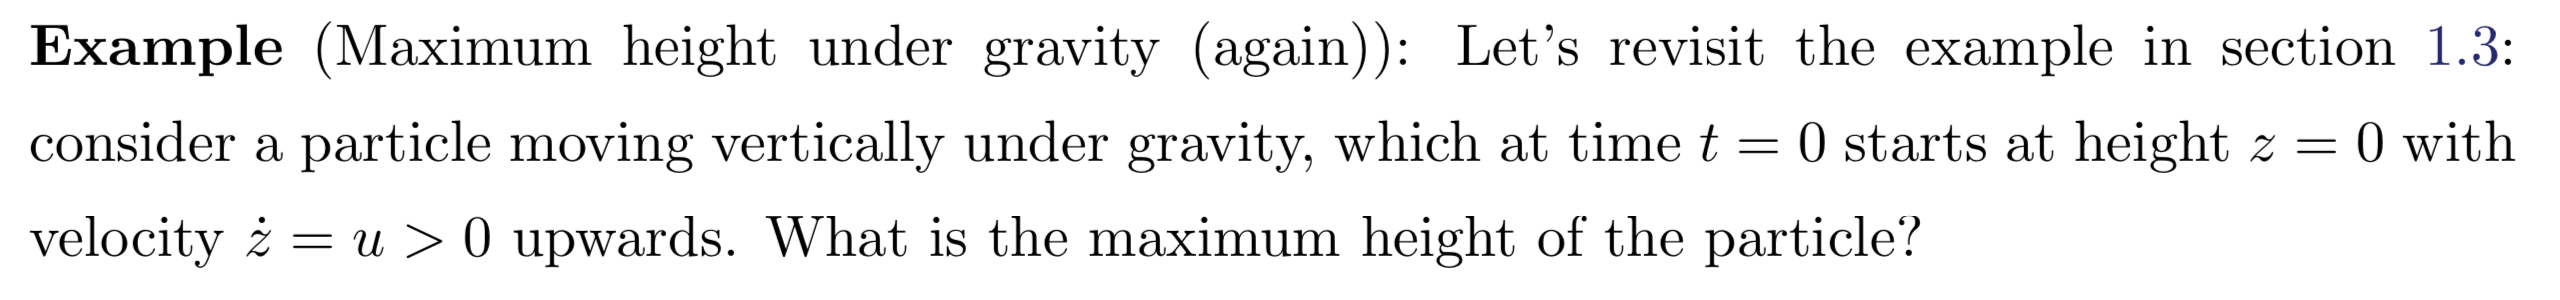
\includegraphics[width=400pt]{img/physics--classical-mechanics--oxford--dynamics--example--gravity.png}
\end{mdframed}

Below we find the maximum height using two methods:
\begin{enumerate}
\item by using Newton's Second Law to write a second-order differential equation for the position
  function, and solving it to give velocity and position functions,
\item by equating the kinetic energy at the beginning with the potential energy at the maximum
  height (when velocity is zero).
\end{enumerate}

Conservation of energy is useful here because total energy ($T + V$) is constant along any
trajectory that satisfies N2L. The logic here is:
\begin{enumerate}
\item We know the trajectory satisfies N2L (because that's how the universe works)
\item Therefore, we know that $T + V$ is constant at any $x$ on the trajectory (one can prove that
  $T+V$ is constant over any trajectory that satisfies N2L.)
\item At one point in the trajectory, we know the values of $T$ and $V$, and the expression for $V$
  involves the quantity of interest $z_{max}$.
\item We also know the values of $T$ and $V$ at another point in the trajectory, not involving
  $z_{max}$.
\item This gives us one equation for the one unknown.
\end{enumerate}

Momentum \textit{is} also conserved, but to see conservation of momentum we have to expand the
system to include the Earth and the particle\footnote{Conservation of momentum is related to N3L,
  and the relevant N3L pair of forces are the Earth's gravitational attraction on the particle and
  the particle's on the Earth, both of which have strength $G\frac{mM_E}{d^2}$, where $M_E$ is the
  mass of the Earth and $d$ is the separation of the two particles, which is approximately the
  radius of the Earth.}. I don't think conservation of momentum can be used to find the height at
which velocity is zero.


We'll use $v_0$ instead of $u$ for the initial velocity.

\begin{enumerate}
\item {\bf Solution via dimensional analysis}\\

  We have
  \begin{align*}
    [g] &= LT^{-2} \\
    [v_0] &= LT^{-1},
  \end{align*}
  and we want $z_{max}$ with units $L$. This suggests that the answer is $z_{max} = C\frac{v_0^2}{g}$,
  where $C$
  is dimensionless.\\
\item {\bf Solution via Newton's Second Law}\\

  Applying N2L here gives $m\ddot{z}(t) = -mg$, i.e.
  \begin{align*}
    \ddot{z}(t) = -g.
  \end{align*}
  Applying FTC once gives the velocity function,
  \begin{align}
    \dot{z}(t) - \dot{z}(0) = \dot{z}(t) - v_0 &= \int_0^t \ddot{z}(t) \dt = -gt \nonumber \\
    \dot{z}(t)                               &= v_0 - gt, \label{oxford-dynamics-example-gravity-velocity}
  \end{align}
  and applying FTC again gives the position function (trajectory),
  \begin{align}
    z(t) - z(0) = z(t) - 0 = \int_0^t \dot{z}(t) \dt = v_0t - \frac{1}{2}gt^2. \label{oxford-dynamics-example-gravity-position}
  \end{align}
  The maximum height occurs when the velocity is zero. From
  \eqref{oxford-dynamics-example-gravity-velocity} we see that this occurs when $t = \frac{v_0}{g}$,
  and from \eqref{oxford-dynamics-example-gravity-position} we see that at that time the height is
  \begin{align*}
    z_{max} = z\(\frac{v_0}{g}\) = \frac{v_0^2}{g} - \frac{1}{2}g\frac{v_0^2}{g^2} = \frac{1}{2}\frac{v_0^2}{g}.
  \end{align*}
\item {\bf Solution via conservation of energy}\\

  Initially, the particle has kinetic energy $T = \frac{1}{2}mv_0^2$.

  Recall that the definition of potential energy relative to $z_0$ is $V(z) = -\int_{z_0}^z F(s) \ds$.

  At its maximum height, gravity has done work
  \begin{align*}
    W = \int_0^{z_{max}} F(z) \dz = \int_0^{z_{max}} m(-g) \dz = -mgz_{max}
  \end{align*}
  on the particle (slowing it down). The potential energy at $z = z_{max}$ relative to $z = 0$ is
  $mgz_{max}$.

  So, we have\\
  \begin{tabular}{l|l|l|}
    Time         & Kinetic energy      & Potential energy \\
    \hline
    $0$          & $\frac{1}{2}mv_0^2$ & 0\\
    $t_{z_{max}}$ & $0$                 & $mgz_{max}$.
  \end{tabular}

  So, from conservation of energy, we have that
  \begin{align*}
    mgz_{max}         &= \frac{1}{2}mv_0^2  \\
    z_{max}           &= \frac{1}{2}\frac{v_0^2}{g}.
  \end{align*}



\end{enumerate}



\section{Force, energy, work, momentum}

Basically, energy measures an accumulation of force over some path in space. Equivalently, the force
at some location in space is a spatial gradient of energy at that location.

However, we also have the Second Law notion that force is the rate of change of momentum,
$F = \dot{p} = m\dot{v}$.

The Second Law is relating force to change in $x$ over time, whereas the notion of energy is
concerned with accumulating force along a spatial trajectory.

Suppose space $x$ is one-dimensional and there is a force $F(x)$ that depends only on position
$x$. We want to compute the integral of force over some interval in space (i.e. ``work''). Let
$v = \dxdt$. Since $F(x) = m\dvdt(x)$, we basically want to compute the following integral:
\begin{align*}
  W = \int_{x_1}^{x_2} \dvdt(x) \dx.
\end{align*}

One approach is to write down the equation $\dvdt = \dxdt \dvdx = v\dvdx$ and thus argue that
\begin{align*}
  W
  = \int_{x_1}^{x_2} v\dvdx \dx
  &= \int_{x_1}^{x_2} v\d v \\
  &= \Big[\frac{1}{2}mv^2\Big]_{v(x_1)}^{v(x_2)},
\end{align*}
where we have ``canceled $\dx$'', and for some reason stopped writing the function argument syntax
``$(x)$''. And why are velocity and acceleration functions of position rather than of time here?
\red{What if the particle visits $x_1$ multiple times with different velocities so that $v(x)$ is
  not well-defined?}

What do these formal manipulations of Leibniz notation actually mean?

Let's go back to the integral we want to compute:
\begin{align*}
  W = \int_{x_1}^{x_2} \dvdt(x) \dx.
\end{align*}
So, we want to calculate the signed area under the graph of $\dvdt(x)$, over the interval
$[x_1, x_2]$.

~\\\hrule~\\

Suppose that we know the trajectory function $x(t)$ of a particle of mass $m$.

Therefore we also know $\dot{x}(t)$ and $\ddot{x}(t)$.

Further, suppose that we know that the net force acting on the particle depends only on its position
$x$. Let this force be $F(x)$.

We want to evaluate
\begin{align*}
  \int_{x_1}^{x_2} F(x) \dx
\end{align*}
in terms of the trajectory function $x(t)$ and its derivatives (velocity and acceleration).

By definition of derivative, at time $t$, the increments $\dx$ and $\dt$ are related according to
$\dx = \dot{x}(t)\dt$, so we can rewrite the integral as
\begin{align*}
  \int_{x_1}^{x_2} F(x(t)) \dot{x}(t)\dt.
\end{align*}
From Newton's Second Law, this is
\begin{align*}
  \int_{x_1}^{x_2} m\ddot{x}(t) \dot{x}(t)\dt,
\end{align*}
or equivalently
\begin{align*}
  \int_{x_1}^{x_2} m\dot{v}(t) v(t)\dt.
\end{align*}
Note that an antiderivative is available here, since $\ddt \frac{1}{2}v^2 = v\dot{v}$. Therefore
\begin{align*}
  \int_{x_1}^{x_2} F(x) \dx = \Big[\frac{1}{2}mv(t)^2\Big]_{t_1}^{t_2},
\end{align*}
where $x(t_1) = x_1$ and $x(t_2) = x_2$. \red{But what if the particle visits $x_1$ multiple times,
  i.e. $x(t_1) = x_1$ has multiple solutions?}



\subsection{Potential energy, conservative force, and work}

The \defn{work} done when a particle moves from $x_0$ to $x_1$ is defined to be
\begin{align*}
  W(x_0 \to x_1) := \int_{x_0}^{x_1} F(x) \dx.
\end{align*}

If this is independent of the path taken between $x_0$ and $x_1$, then we say the force is
\defn{conservative} and define the \defn{potential energy} at $x$, relative to $x_0$ to be
\begin{align*}
  V(x) &:= -\int_{x_0}^x F(x') \dx'.
\end{align*}
If the integral depends on the path taken, the potential energy is undefined.

\blue{A force moves something in space (causes an acceleration). Equivalently, something moves in
  space because a small displacement in some direction is associated with a lower potential
  energy. In fact, the force at a location \emph{is} the gradient in potential energy at that
  location.}

\begin{align*}
  F(x) &= -\frac{\d V(x)}{\dx} \\
  V(x) &= -\int_{x_0}^x F(x') \dx'
\end{align*}

\todo{Understand this}:

A force that depends only on position in one dimension is always conservative, because the integral
depends only on the endpoints. But a force that depends on e.g. time or velocity is
non-conservative. Friction is such a force because although it looks like a constant force
($\mu mg$), its direction (sign) is the opposite of the direction of velocity, so it is in fact
velocity-dependent.

Also, how is this so:
\begin{quote}
  \emph{Since friction always opposes the motion, the contributions to the $W = \int F \dx$ integral are
    always negative, so there is never any cancellation. The result is therefore a large negative
    number.}
\end{quote}

\subsection{Slowing down a moving object}

Facts:

\begin{enumerate}
\item The rate of change of momentum is determined by the net force acting on an object.
\item To slow something down, a force must be applied for some period of time.
\item To slow something which has momentum $p$, a strong force could be applied briefly, or a weaker
  force for a longer time.
\item ``Slow something down'' in those sentences could be replaced with ``change the velocity''. The
  change in velocity could be a change in direction, without a change in speed.
\end{enumerate}


Consider two bodies traveling in one dimension with masses and velocities $m_1, v_1$ and $m_2,
v_2$. Their momenta are identical: $m_1v_1 = m_2v_2$.

Suppose that mass $m_1 > m_2$, and therefore $v_1 < v_2$.

A force $F$ acts to slow them down. Over what length of time must the force be in effect?

The force causes accelerations (decelerations) $a_1 = F/m_1$ and $a_2 = F/m_2$. So we have velocity
functions
\begin{align*}
  \dv{x_1}{t} (t) &= v_1 - \frac{F}{m_1}t \\
  \dv{x_2}{t} (t) &= v_2 - \frac{F}{m_1}t,
\end{align*}
and we see that the velocities become equal to zero at the same time, i.e. when
$t = \frac{m_1v_1}{F} = \frac{m_2v_2}{F}$.

So, \blue{the length of time for which a force must be applied depends only on the momentum}; not on the
mass or velocity separately.

Now, how far does a mass travel while it is slowing down (i.e. over time $mv/F$)? This is
\begin{align*}
  x &= \int_{t=0}^{t=mv/F} \(v - \frac{F}{m}t\) \dt \\
    &= vt - \frac{F}{2m}t^2\Big|_{t=0}^{t=mv/F} \\
    &= \frac{mv^2}{F} - \frac{F}{2m}\frac{m^2v^2}{F^2} \\
    &= \frac{1}{2}mv^2/F.
\end{align*}

So, in order for a constant force $F$ to halt a mass $m$ with velocity $v$, the product of force and
the distance over which the force is applied (i.e. the work done) must equal the kinetic energy of
the mass $\frac{1}{2}mv^2$.

I.e. \blue{the distance over which the force must be applied depends on the kinetic energy}
$\frac{1}{2}mv^2$.

The lighter mass covers more distance while it is slowing down, because it has higher kinetic energy.

The following connections between force and momentum, and force and work/energy, make sense under
the FTC:
\begin{enumerate}
\item Force is the time derivative of momentum. The integral of force over time corresponds to change in momentum.
\item Force is the spatial derivative of potential energy. The integral of force over space
  (i.e. work) corresponds to change in potential energy.
\end{enumerate}



\subsection{Example: gravitational potential energy}

Consider two point masses $M$ and $m$, separated by a distance $r$. Newton's law of gravitation
states that there is a force between them of magnitude $-GMm/r^2$ (the force is attractive, hence
the negative sign).

The potential energy of the system at separation $r$, relative to separation $r_0$, is

\begin{align*}
  V(r) &= -\int_{r_0}^r F(r) \dr \\
       &= -\int_{r_0}^r \frac{-GMm}{r^2} \dr \\
       &= -\(\frac{GMm}{r} - \frac{GMm}{r_0}\).
\end{align*}

Typically in this situation we would choose $r_0 = \infty$ as the reference separation, so that
\begin{align*}
  V(r) = -\frac{GMm}{r}.
\end{align*}

\blue{Potential energy, relative to $r = \infty$, decreases as the two masses get closer: so the
  masses will approach each other. It's always negative because we have measured it relative to
  $r = \infty$, and any separation is more favorable than infinitely large separation.}

\begin{question*}
  What is the gravitational potential energy of a mass $m$ at a height $y$, relative to the Earth's
  surface?
\end{question*}

\begin{proof}
  Let the mass and radius of Earth be $M$ and $R$. Then
  \begin{align*}
    V(y) &= -\(\frac{GMm}{R + y} - \frac{GMm}{R}\) \\
         &= GMm(\frac{R + y - R}{R^2 + Ry}) \\
   &\approx \frac{GMmy}{R^2},
  \end{align*}
  for $y << R$. Recall that the gravitational acceleration of a particle of mass $m$ is $g = \frac{GM}{R^2}$. So
  we can write this in terms of $g$ as
  \begin{align*}
  V(y) &\approx mgy.
  \end{align*}
\end{proof}
\blue{This expression for potential energy decreases as the height $y$ decreases. It does still
  depend on the inverse of the spatial separation, but this factor is approximately constant since
  $y << R$. In any case, the mass falls to Earth, since smaller $y$ has lower potential energy. The
  derivative of the potential energy is the familiar gravitational force
  \begin{align*}
    mg = \frac{GMm}{R^2}.
  \end{align*}
}

\section{Gravity}

\begin{tabular*}{1.0\linewidth}{l|l}
  $M, m$ & masses of two bodies \\
  $r$    & distance between bodies
\end{tabular*}

Newton's law of gravity: the force between two bodies is $F = G\frac{Mm}{r^2}$, where $G$ is the
gravitational constant.

Units: since $[F] = \frac{LM}{T^2}$, we have $[G] = \frac{LM}{T^2}\frac{L^2}{M^2} = \frac{L^3}{MT^2}$.

\begin{tabular*}{1.0\linewidth}{l|l}
  $M_E = 5.972 \times 10^{24} kg$ & mass of the Earth \\
  $R =  6.371 \times 10^6 m$     & radius of the Earth \\
  $G = 6.67408 \times 10^{-11} m^3 kg^{-1} s^{-2}$        & gravitational constant\\
  $m$ & mass of an object
\end{tabular*}

The acceleration of the object due to gravity at the Earth's surface is
\begin{align*}
  g
  = \frac{F}{m}
  = G\frac{M_E}{R^2}
  = \frac{6.67408 \times 10^{-11} \times 5.972 \times 10^{24}}{(6.371 \times 10^6)^2}
  = 9.82 ms^{-2}.
\end{align*}

\blue{Note that, for gravity, the strength of the force itself depends on the mass $m$. So Newton's
  Second Law for a body of mass $m$ near the Earth's surface is
\begin{align*}
  ma &= F \\
  ma &= mg \\
  a  &= g.
\end{align*}
}



\subsection*{Conservation of momentum}

The basic argument for conservation of momentum derives from Newton's 3rd law:

Suppose particle $a$ is exerting a force $\vec{F}_{ab}$ on particle $b$. Since
$\vec{F} = \dv{\vec{p}}{t}$, we have that
\begin{align*}
  \int_{t=0}^t \vec{F}_{ab} \dt = \vec{p_b(t)} - \vec{p_b(0)}.
\end{align*}
From Newton's Third Law we have $\vec{F}_{ab} = -\vec{F}_{ba}$, which implies
$\vec{p_b(t)} - \vec{p_b(0)} = -\(\vec{p_a(t)} - \vec{p_a(0)}\)$ and therefore
\begin{align*}
  \vec{p_a(t)} + \vec{p_b(t)} &= \vec{p_a(0)} + \vec{p_b(0)},
\end{align*}
i.e. total momentum is conserved.



\subsection*{Collisions in 1-D}

A collision between two particles may be
\begin{itemize}
\item \defn{inelastic}: kinetic energy is lost, e.g. lumps of putty.\footnote{Taylor 3.1 Ex 3.1 p.84, }
\item \defn{elastic}: kinetic energy is conserved, e.g. billiard balls\footnote{Taylor ch4 p. 142, Morin 5.6 p.162 (using CM frame), Morin 5.7 p.164 (using conservation of KE)}
\end{itemize}

\subsubsection*{Perfectly inelastic collision\footnote{Taylor 3.1 p.84}}

The simplest case seems to be ``perfectly inelastic'' collision: two lumps of putty that stick
together (without generating any heat or sound). In this case we have one unknown (the
post-collision velocity), and one equation (conservation of momentum) suffices.

\red{Is kinetic energy conserved here? If not why not?}

\begin{mdframed}
  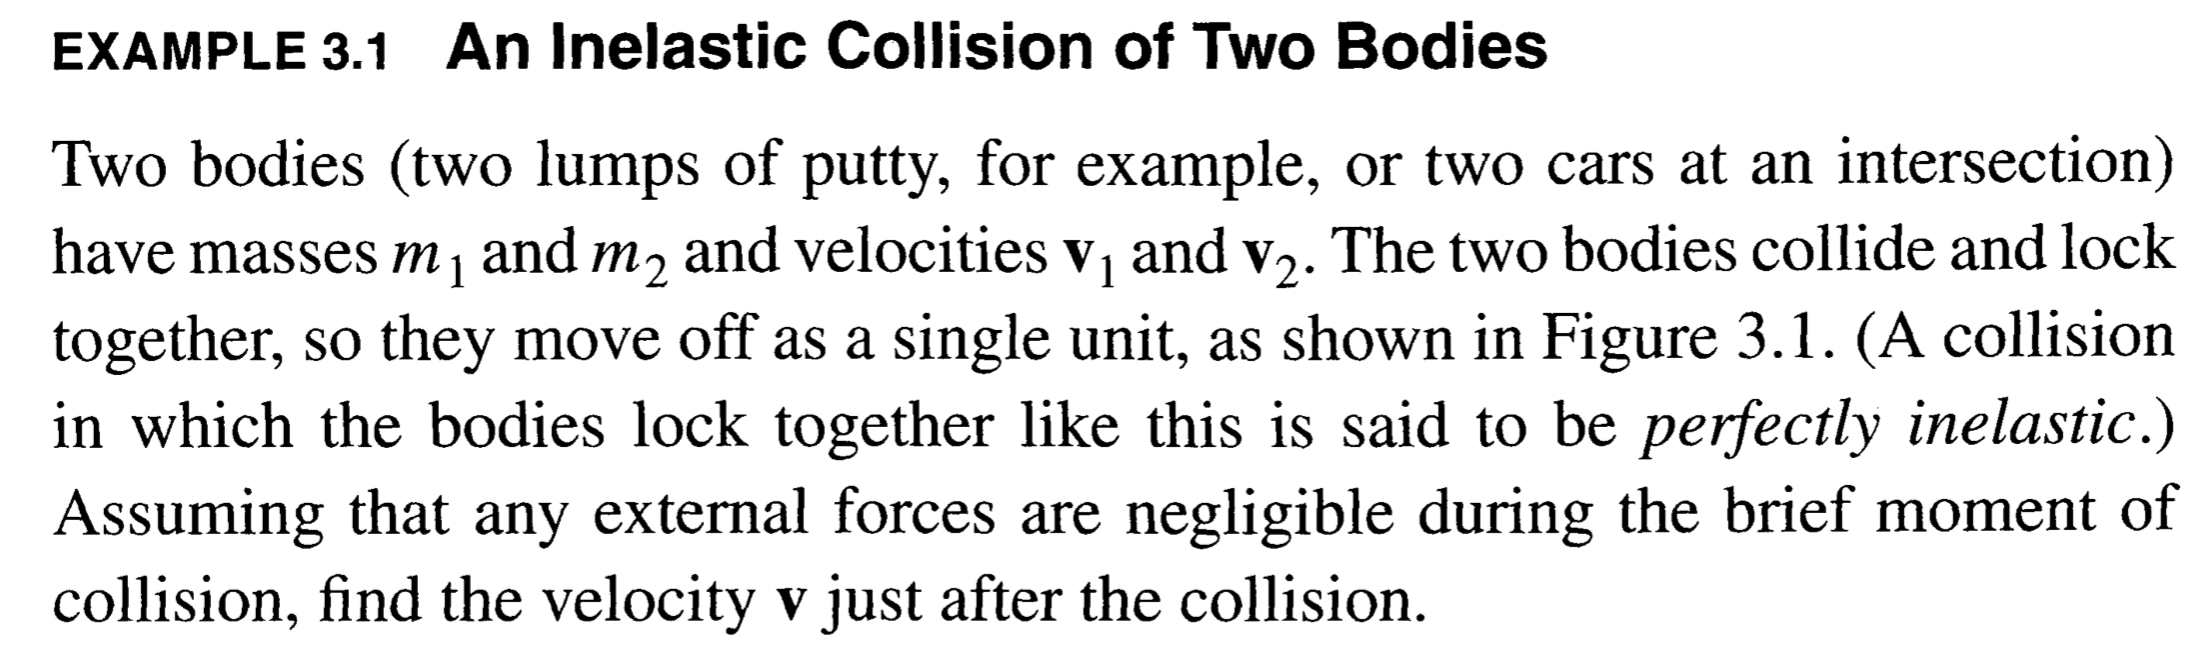
\includegraphics[width=400pt]{img/physics--classical-mechanics--taylor--sec-3-1.png}
\end{mdframed}

We have
\begin{align*}
  m_1\vec{v_1} + m_2\vec{v_2} &= (m_1 + m_2)\vec{v} \\
  \vec{v} &= \frac{m_1\vec{v_1} + m_2\vec{v_2}}{m_1 + m_2} \\
          &= \alpha\vec{v_1} + (1 - \alpha)\vec{v_2},
\end{align*}
where $\alpha = \frac{m_1}{m_1 + m_2}$.


\red{What happens if we do this with conservation of energy? Suppose we are in 1-D}
\begin{align*}
  \frac{1}{2}m_1v_1^2 + \frac{1}{2}m_2v_2^2 &= \frac{1}{2}(m_1 + m_2)v^2 \\
  v                                        &= \sqrt{\frac{m_1v_1^2 + m_2v_2^2}{m_1 + m_2}}.
\end{align*}
So, letting $v_M$ and $v_E$ be the momentum- and energy- based post-collision velocity answers, we
have
\begin{align*}
  v_E^2 &= \alpha v_1^2 + (1 - \alpha)v_2^2 \\
  v_M^2 &= \(\alpha v_1 + (1 - \alpha)v_2\)^2.
\end{align*}
Since $x \mapsto x^2$ is a convex function (\ref{convexity}), we have that $v_E > v_M$.

\red{Why is this -- why does assuming conservation of kinetic energy lead to a higher post-collision
  velocity than assuming conservation of momentum?}  \blue{Is this because squashing the lumps of
  putty together necessarily loses KE, so if we assume KE is conserved then we are overestimating
  the post-collision KE, which is why the post-collision velocity $v_E$ is greater than the estimate
  $v_M$ based on conservation of momentum?}




\subsubsection*{Example: Elastic collision (Morin p.162)}

\begin{mdframed}
  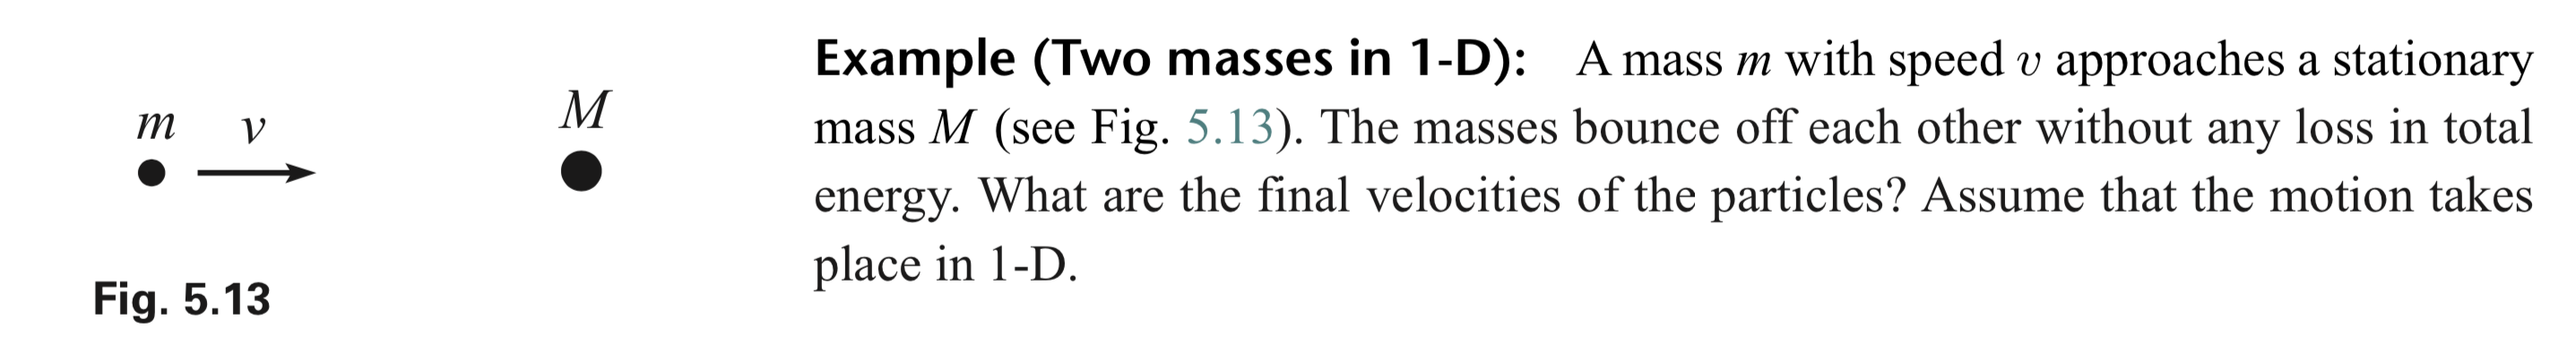
\includegraphics[width=400pt]{img/physics--classical-mechanics--morin--sec-5-6-ex.png}
\end{mdframed}

This can be solved in two ways:
\begin{enumerate}
\item Using the center of mass (CM) frame (Morin p.162)
\item Using conservation of kinetic energy (Morin p. 164, )
\end{enumerate}

Let the post-collision masses and velocities be $(m, v_f)$ and $(M, V_f)$.

{\bf Solution using conservation of kinetic energy}\\

From conservation of momentum and KE we have the system of equations
\begin{align}
  mv              &= mv_f + MV_f \\
  \frac{1}{2}mv^2 &= \frac{1}{2}mv_f^2 + \frac{1}{2}MV_f^2.
\end{align}
Now, we solve for $v_f$ and $V_f$...

\begin{verbatim}
#+begin_src mathematica :results raw pp
Solve[m v == m vf + M Vf && m v^2 == m vf^2 + M Vf^2, {vf, Vf}]
#+end_src

#+RESULTS:
: {{vf -> v, Vf -> 0}, {vf -> (m*v - M*v)/(m + M), Vf -> (2*m*v)/(m + M)}}
\end{verbatim}
...and the solution is
\begin{align*}
  v_f &= \frac{mv - Mv}{m + M} \\
  V_f &= \frac{2mv}{m + M}.
\end{align*}

So the stationary mass moves in the direction of impact, and for the moving mass:
\begin{itemize}
\item if it's smaller, it reverses its direction,
\item if it's the same mass, it stops dead,
\item if it's larger, it continues in the same direction.
\end{itemize}
Furthermore, the stationary mass always moves away faster than the moving mass. For values of the
stationary mass approaching zero, the ratio of their speeds approaches 2.


Now\footnote{\url{https://www.youtube.com/watch?v=HEfHFsfGXjs}}, what about if they are both in
motion when they collide? In that case we have
\begin{align}
  mv + MV                           &= mv_f + MV_f \\
  \frac{1}{2}mv^2 + \frac{1}{2}MV^2 &= \frac{1}{2}mv_f^2 + \frac{1}{2}MV_f^2.
\end{align}
\begin{verbatim}
#+begin_src mathematica :results raw pp
Solve[m v + M V == m vf + M Vf && m v^2 + M V^2 == m vf^2 + M Vf^2, {vf, Vf}]
#+end_src

#+RESULTS:
: {{vf -> v, Vf -> V}, {vf -> (m*v - M*v + 2*M*V)/(m + M), Vf -> (2*m*v - m*V + M*V)/(m + M)}}
\end{verbatim}
\begin{align*}
  v_f &= \frac{mv - Mv + 2MV}{m + M} \\
  V_f &= \frac{2mv - mV + MV}{m + M}.
\end{align*}

\newpage
The 3blue1brown $\pi$ in colliding blocks
video\footnote{\url{https://www.youtube.com/watch?v=HEfHFsfGXjs}} involves perfectly elastic
collisions of two blocks, and a wall. The block closest to the wall starts off stationary, and the
outer block (mass $m_1$) moves towards it with constant velocity. We count the number of collisions
between blocks, and between the inner block and the wall, for varying values of the mass $m_1$ of
the outer block.

\begin{minted}{python3}
import sys
from dataclasses import dataclass
from typing import Tuple


@dataclass
class Blocks:
    m0 = 1.0  # mass of left block
    m1 = None  # mass of right block (supplied as input)

    v0 = 0.0  # left block starts off stationary
    v1 = -1.0  # initial velocity of right block

    def will_collide_again(self):
        return abs(self.v0) > self.v1

    def collide(self):
        v0, v1 = self.v0, self.v1
        m0, m1 = self.m0, self.m1
        self.v0 = (m0 * v0 - m1 * v0 + 2 * m1 * v1) / (m0 + m1)
        self.v1 = (2 * m0 * v0 - m0 * v1 + m1 * v1) / (m0 + m1)

    def simulate(self):
        n = 0
        while True:
            self.collide()
            n += 1
            if self.will_collide_again():
                # Bounce off wall
                self.v0 = -self.v0
                n += 1
            else:
                break
        if self.v0 < 0:
            # Bounce off wall
            n += 1
        print(n)


if __name__ == "__main__":
    assert not sys.argv[2:]
    blocks = Blocks()
    blocks.m1 = float(sys.argv[1])
    blocks.simulate()
\end{minted}

Here are the counts for $m_1$ taking values that are integer powers of 100:

\begin{verbatim}
$ for i in 0 1 2 3 4 5 6; do python 3blue1brown-blocks.py $((100**i)); done
3
31
314
3141
31415
314159
3141592
\end{verbatim}

\section{Projectile motion}

A projectile of mass $m$ is released with velocity $v_0$ at an angle $\theta$ to the ground. There
is no air resistance.

Note that vertical and horizontal motion are independent of each other. The equations of motion are:

\begin{itemize}
\item {\bf Vertical}\\
  $\ddot{y}(t) = -g$, with initial condition $\dot{y}(0) = v_0\sin\theta$.
\end{itemize}

\subsection{Using integration / FTC to solve the equation of motion}
Informally, since the acceleration is constant, the solution for the velocity function must be
$\dot{y}(t) = v_0\sin\theta - gt$, and therefore by integration the solution for vertical
position is $y(t) = y_0 + v_0\sin\theta t -\frac{1}{2}gt^2$.

More formally, we want to identify the set of functions $y$ that are consistent with the facts:
\begin{align*}
  \ddot{y}(t) &= -g \\
  \dot{y}(0)  &= v_0 \\
  y(0)        &= y_0.
\end{align*}

The first step is to identify the set of first-derivative functions $\dot{y}$ that fit the
facts. Using only the fact that the second derivative is a constant $-g$, we conclude that the
first derivative can be any linear function: $\dot{y}(t) = C - gt$. Then using the initial
velocity, we narrow this further to $\dot{y}(t) = v_0 - gt$.

More formally... the ``antiderivative'' operation maps a single function to a (infinite) set of
functions.
\begin{align*}
  \int \ddot{y}(t) \dt = \int -g \dt = C - gt.
\end{align*}

But the operation of integration maps an $\R \to \R$ function to $\R$.

We have an $\R \to \R$ function $\ddot{y}(t) = -g$. Antidifferentiating tells us that a family of
linear velocity functions are consistent with the acceleration function. What does integration
tell us? It tells us the ``net amount'' of acceleration that has accumulated between time $0$ and
time $t$. (And the FTC tells us that antidifferentiating gives us a trick to find this net amount
easily.)

It's easier to think about velocity and distance. ``Net amount of accumulated velocity'',
i.e. area under the velocity graph, corresponds to net displacement. E.g. $70$ mph $\times$ $2$
hrs equals $140$ miles displacement. What does that familiar calculation correspond to formally?
$140$ miles displacement is saying $x(2) - x(0) = 140$. So the statement is that
\begin{align}
    x(t) - x(0) &= \int_{t'=0}^{t'=t} \dxdt(t') \dt' \label{pcm-ftc} \\
                &= \int_{t'=0}^{t'=t} 70 \dt'.       \nonumber
\end{align}
In this case, \eqref{pcm-ftc} is common sense, because the velocity is constant. But for an
arbitrary velocity function, it would be invoking the FTC.

To compute that integral we can either
\begin{enumerate}
\item Use common sense again: visualize it as the area of a rectangle with height $70$ and width
  $t$.
\item Invoke the FTC a second time: notice that area is increasing linearly with $t$ with a slope
  of $70$, so the answer to the integral is given by the difference in value at $0$ and at $t$ of
  some function which has a slope equal to the integrand. Obvious for a constant integrand, but
  the FTC says that that line of thought still holds when the integrand is any well-behaved
  function. In other words, we need to antidifferentiate: find a function that has derivative
  $70$. In other words, we need to solve a differential equation: $f' = 70$.
\end{enumerate}

So in the velocity/distance problem, the facts were
\begin{align*}
    \dot{x} &= 70 \\
    x(0)    &= 0,
\end{align*}
we wanted to know the function $x$, and we found the solution $x(t) = 70t$ by solving the equation
\begin{align*}
    x(t) - x(0) = \int_0^t 70 \dt.
\end{align*}

Returning to the vertical acceleration of the projectile, the area under the acceleration graph
corresponds to net change in velocity. Recall that the facts are
\begin{align*}
    \ddot{y}(t) &= -g \\
    \dot{y}(0)  &= v_0 \\
    y(0)        &= y_0.
  \end{align*}
  We want to know the function $y$. So, invoking the FTC, we write down the equation
  \begin{align*}
    \int_{t'=0}^{t'=t}\ddot{y}(t') \dt' &= \dot{y}(t) - \dot{y}(0) \\
    \int_{t'=0}^{t'=t}-g \dt' &= \dot{y}(t) - v_0.
\end{align*}
Then, to solve this equation, we invoke FTC again, identifying $-gt$ as an antiderivative, and
conclude that
\begin{align*}
    -gt'\Big|_{t'=0}^{t'=t} &= \dot{y}(t) - v_0 \\
    \dot{y}(t)                   &= v_0 - gt.
\end{align*}
Then, we repeat the procedure, writing down
\begin{align*}
    \int_{t'=0}^{t'=t}\dot{y}(t') \dt' &= y(t) - y(0) \\
    \int_{t'=0}^{t'=t}v_0 - gt \dt'    &= y(t) - y_0 \\
    v_0t' - \frac{1}{2}gt'^2\Big|_{t'=0}^{t'=t} &= y(t) - y_0 \\
    y(t) &= y_0 + v_0t - \frac{1}{2}gt^2.
\end{align*}
